\documentclass[a4paper,12pt]{extarticle}
\usepackage[utf8x]{inputenc}
\usepackage[T1,T2A]{fontenc}
\usepackage[russian]{babel}
\usepackage{hyperref}
\usepackage{indentfirst}
\usepackage{listings}
\usepackage{color}
\usepackage{here}
\usepackage{array}
\usepackage{multirow}
\usepackage{graphicx}
\usepackage{amsmath}
\usepackage{amssymb}

\usepackage{caption}
\renewcommand{\lstlistingname}{Программа} % заголовок листингов кода

\bibliographystyle{ugost2008ls}

\usepackage{listings}
\lstset{ %
extendedchars=\true,
keepspaces=true,
language=C,						% choose the language of the code
basicstyle=\footnotesize,		% the size of the fonts that are used for the code
numbers=left,					% where to put the line-numbers
numberstyle=\footnotesize,		% the size of the fonts that are used for the line-numbers
stepnumber=1,					% the step between two line-numbers. If it is 1 each line will be numbered
numbersep=5pt,					% how far the line-numbers are from the code
backgroundcolor=\color{white},	% choose the background color. You must add \usepackage{color}
showspaces=false				% show spaces adding particular underscores
showstringspaces=false,			% underline spaces within strings
showtabs=false,					% show tabs within strings adding particular underscores
frame=single,           		% adds a frame around the code
tabsize=2,						% sets default tabsize to 2 spaces
captionpos=t,					% sets the caption-position to top
breaklines=true,				% sets automatic line breaking
breakatwhitespace=false,		% sets if automatic breaks should only happen at whitespace
escapeinside={\%*}{*)},			% if you want to add a comment within your code
postbreak=\raisebox{0ex}[0ex][0ex]{\ensuremath{\color{red}\hookrightarrow\space}},
texcl=true,
inputpath=listings,                     % директория с листингами
}

\usepackage[left=2cm,right=2cm,
top=2cm,bottom=2cm,bindingoffset=0cm]{geometry}

%% Нумерация картинок по секциям
\usepackage{chngcntr}
\counterwithin{figure}{subsection}
\counterwithin{table}{section}

%%Точки нумерации заголовков
\usepackage{titlesec}
\titlelabel{\thetitle.\quad}
\usepackage[dotinlabels]{titletoc}

%% Оформления подписи рисунка
\addto\captionsrussian{\renewcommand{\figurename}{Рис.}}
\captionsetup[figure]{labelsep = period}

%% Подпись таблицы
\DeclareCaptionFormat{hfillstart}{\hfill#1#2#3\par}
\captionsetup[table]{format=hfillstart,labelsep=newline,justification=centering,skip=-10pt,textfont=bf}

%% Путь к каталогу с рисунками
\graphicspath{{fig/}}

\setcounter{tocdepth}{3}

\begin{document}	% начало документа

% Титульная страница
\begin{titlepage}	% начало титульной страницы

	\begin{center}		% выравнивание по центру

		\large Санкт-Петербургский Политехнический Университет Петра Великого\\
		\large Институт компьютерных наук и технологий \\
		\large Кафедра компьютерных систем и программных технологий\\[6cm]
		% название института, затем отступ 6см
		
		\huge Телекоммуникационные технологии\\[0.5cm] % название работы, затем отступ 0,5см
		\large Отчет по лабораторной работе №5\\[0.1cm]
		\large Частотная и фазовая модуляция\\[5cm]

	\end{center}


	\begin{flushright} % выравнивание по правому краю
		\begin{minipage}{0.25\textwidth} % врезка в половину ширины текста
			\begin{flushleft} % выровнять её содержимое по левому краю

				\large\textbf{Работу выполнил:}\\
				\large Болдырев А.В.\\
				\large {Группа:} 33501/3\\
				
				\large \textbf{Преподаватель:}\\
				\large Богач Н.В.

			\end{flushleft}
		\end{minipage}
	\end{flushright}
	
	\vfill % заполнить всё доступное ниже пространство

	\begin{center}
	\large Санкт-Петербург\\
	\large \the\year % вывести дату
	\end{center} % закончить выравнивание по центру

\thispagestyle{empty} % не нумеровать страницу
\end{titlepage} % конец титульной страницы

\vfill % заполнить всё доступное ниже пространство

% Содержание
% Содержание
\renewcommand\contentsname{\centerline{Содержание}}
\tableofcontents
\newpage


\section{Цель работы}
Изучение частотной и фазовой модуляции/демодуляции сигнала.
\section{Постановка задачи}
Сгенерировать однотональный сигнал низкой частоты, выполнить фазовую модуляцию/демодуляцию, частотную модуляцию/демодуляцию. Посмотреть, как модуляция влияет на спектр сигнала.

\section{Теоретическая информация}

\subsection{Модуляция}
Сигналы от любых источников информации передаются по линиям связи к приемникам, например, в измерительно-вычислительные системы регистрации и обработки данных. Как правило, информационные сигналы являются низкочастотными и ограниченными по ширине спектра, тогда как методы передачи сигналов рассчитаны на работу с высокочастотным сигналом. При этом важным вопросом является частотное разделение каналов передачи информации с целью эффективного использования каналообразующего оборудования и выделенного для передачи частотного диапазона. Перенос спектра сигналов из низкочастотной области на заданную частоту, т.е. в выделенную для их передачи область высоких частот выполняется операцией \textit{модуляции}. Обозначим низкочастотный сигнал, подлежащий передаче по какому-либо каналу связи, $s(t)$ .   

В канале связи для передачи данного сигнала выделяется определенный диапазон высоких частот и формируется вспомогательный периодический высокочастотный сигнал $u(t)   =   f(t;   a_1,   a_2,   ...   a_m)$. Совокупность параметров $a_i$ определяет форму вспомогательного сигнала. Значения параметров $a_i$ в отсутствие модуляции являются величинами постоянными. Если на один из этих параметров перенести сигнал $s(t)$, т.е. сделать его значение пропорционально зависимым от значения $s(t)$ во времени (или по любой другой независимой переменной), то форма сигнала $u(t)$ приобретает новое свойство. Она служит для переноса информации, содержащейся в сигнале $s(t)$. Сигнал $u(t)$ называется \textit{несущим сигналом}, \textit{несущим колебанием} или просто \textit{несущей}  ($carrier$),  а физический процесс переноса информации на
параметры несущего сигнала     –     его \textit{модуляцией}. 

Исходный информационный сигнал $s(t)$ называют \textit{модулирующим}, результат модуляции    –    \textit{модулированным сигналом}. Обратную операцию выделения модулирующего сигнала из модулированного колебания называют демодуляцией или детектированием.

\subsection{Генерация однотонального низкочастотного сигнала $s(t)$}
Для генерации гармонического сигнала воспользуемся формулой $s(t) = A*cos(2*\pi * f*t + \varphi)$, где А - амплитуда сигнала, f - частота, t - вектор отсчетов времени, $\varphi$ - смещение по фазе.

\subsection{Типы модуляции}
\subsubsection{Фазовая модуляция}
При фазовой модуляции (phase modulation – PM) значение фазового угла постоянной несущей частоты колебаний $\omega_0$ пропорционально амплитуде модулирующего сигнала $s(t)$. Соответственно, уравнение ФМ–сигнала определяется выражением: 
\begin{equation}
	u(t) = U_m cos(\omega_0 t + k s(t))
\end{equation}
Сигнал после фазовой модуляции имеет максимальную частоту в точке, где максимально значение производной несущего сигнала (аналогично для минимума частоты).

\subsubsection{Угловая модуляция}
При угловой модуляции в несущем гармоническом колебании $u(t) = U_m cos(\omega t + \varphi)$  значение амплитуды колебаний $U_m$ остается постоянным, а информация $s(t)$ переносится либо на частоту $\omega$, либо на фазовый угол $\varphi$. В обоих случаях текущее значение фазового угла гармонического колебания $u(t)$ определяет аргумент $\psi (t) = \omega t + \varphi$ , который называется \textit{полной фазой} колебания.
Частотная модуляция выполняется по закону: 
\begin{equation}
	u(t) = U_m cos(\omega_0 t + k \int_{0}^{t} s(t) dt)
\end{equation}

Изображение сигнала после угловой модуляции приведено ниже на риунке \ref{pic:Freq_mod_theor} :
\begin{figure}[H]
	\begin{center}
		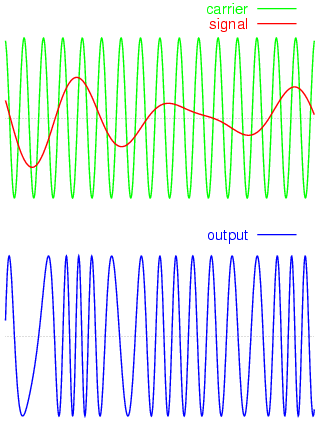
\includegraphics[scale=0.7]{Freq_mod_theor}
		\caption{Угловая модуляция сигнала} 
		\label{pic:Freq_mod_theor} % название для ссылок внутри кода
	\end{center}
\end{figure}

Данный вид модуляции внешне совпадает с фазовой, на практике необходимо иметь априорную информацию о типе модуляции при решении задачи демодуляции.


\section{Ход работы}
Код программы представлен ниже - два листинга, относящихся к фазовой модуляции и один относящийся к частотной модуляции \ref{code:code_1} , \ref{code:Phasemod} , \ref{code:Freqmod} : 
\lstinputlisting[
	label=code:code_1,
	caption={Код в МатЛаб},% для печати символ '_' требует выходной символ '\'
]{Code_1.m}
\lstinputlisting[
	label=code:Phasemod,
	caption={Код в МатЛаб},% для печати символ '_' требует выходной символ '\'
]{Phasemod.m}
В коде применены функции pmmod и pmdemod.
Далее приведен листинг кода частотной модуляции:
\lstinputlisting[
	label=code:Freqmod,
	caption={Код в МатЛаб},% для печати символ '_' требует выходной символ '\'
]{Freqmod.m}
В коде применены функции fmmod и fmdemod.

\subsection{Генерация однотонального сигнала}
Для начала получим обычный гармонический сигнал. Сгенерированный сигнал представлен на рисунке \ref{pic:signal_one_tone}:
\begin{figure}[H]
	\begin{center}
		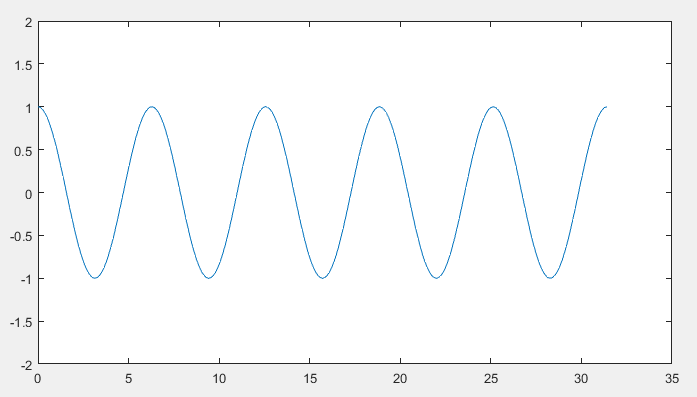
\includegraphics[scale=0.7]{signal_one_tone}
		\caption{Гармонический сигнал $s(t) = A*cos(2*\pi * f*t + \varphi)$} 
		\label{pic:signal_one_tone} % название для ссылок внутри кода
	\end{center}
\end{figure}
Для однотонального сигнала спектр выглядит следующим образом:
\begin{figure}[H]
	\begin{center}
		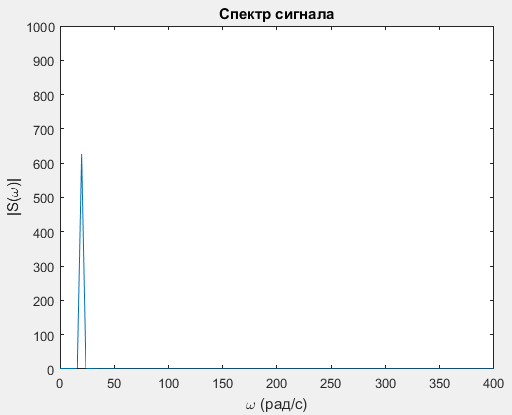
\includegraphics[scale=0.7]{signal_one_tone_spec}
		\caption{Спектр гармонического сигнала $s(t) = A*cos(2*\pi * f*t + \varphi)$} 
		\label{pic:signal_one_tone_spec} % название для ссылок внутри кода
	\end{center}
\end{figure}

\subsection{Частотная модуляция}

\begin{figure}[H]
	\begin{center}
		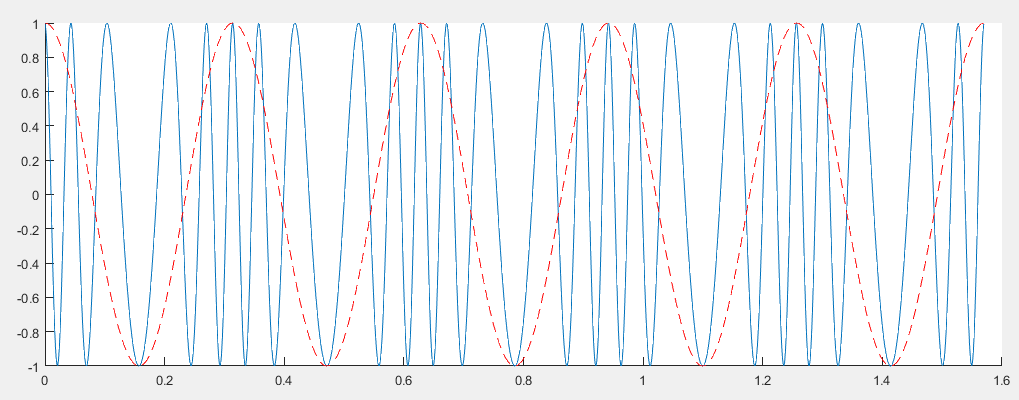
\includegraphics[scale=0.7]{freq_mod_sig_1000_0}
		\caption{Частотно-модулированный сигнал} 
		\label{pic:freq_mod_sig_1000_0} % название для ссылок внутри кода
	\end{center}
\end{figure}
\begin{figure}[H]
	\begin{center}
		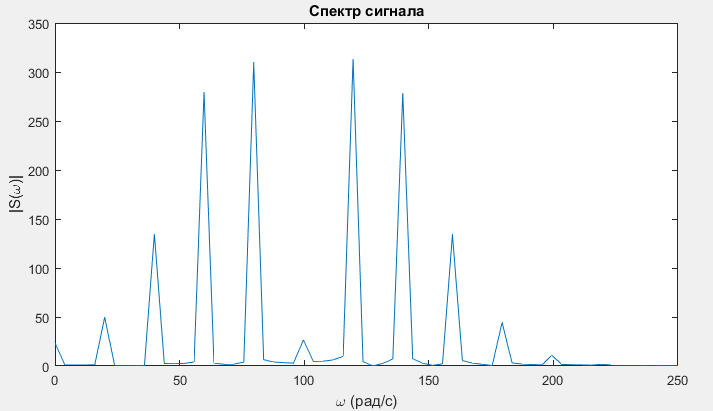
\includegraphics[scale=0.7]{freq_mod_sig_spec_1000_0}
		\caption{Спектр частотно-модулированного сигнала} 
		\label{pic:freq_mod_sig_spec_1000_0} % название для ссылок внутри кода
	\end{center}
\end{figure}

\subsection{Фазовая модуляция}

\begin{figure}[H]
	\begin{center}
		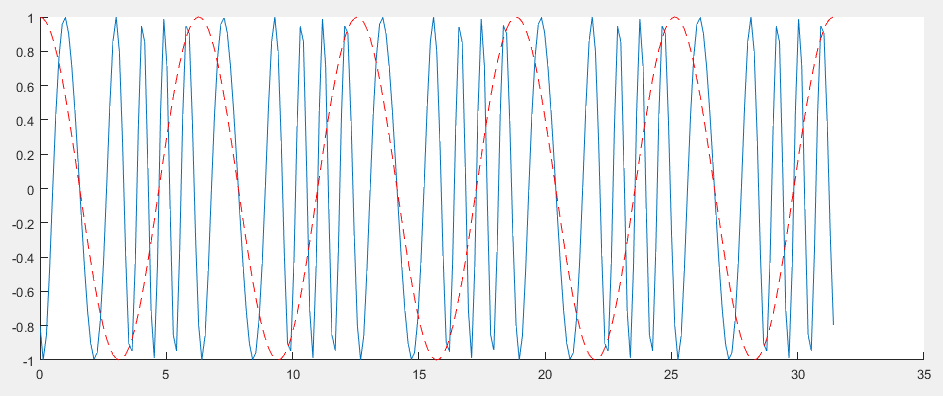
\includegraphics[scale=0.7]{phase_mod_sig_carr}
		\caption{Фазово-модулированный сигнал (с отображением несущей гармоники)} 
		\label{pic:phase_mod_sig_carr} % название для ссылок внутри кода
	\end{center}
\end{figure}

\begin{figure}[H]
	\begin{center}
		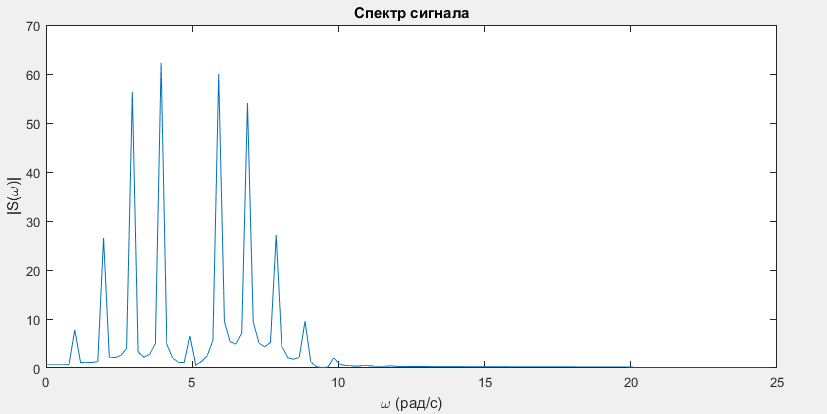
\includegraphics[scale=0.7]{phase_mod_sig_carr_spec}
		\caption{Спектр фазово-модулированного сигнала} 
		\label{pic:phase_mod_sig_carr_spec} % название для ссылок внутри кода
	\end{center}
\end{figure}

\subsection{Демодуляция ЧМ и ФМ}
Произведем демодуляцию модулированных сигналов.
\begin{figure}[H]
	\begin{center}
		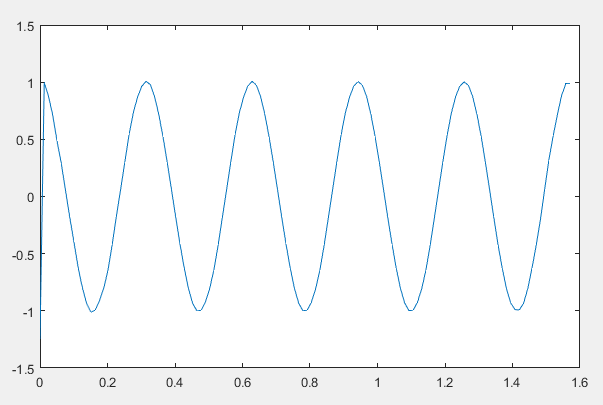
\includegraphics[scale=0.7]{phase_demod_sig}
		\caption{Фазово-демодулированный сигнал} 
		\label{pic:phase_demod_sig} % название для ссылок внутри кода
	\end{center}
\end{figure}
\begin{figure}[H]
	\begin{center}
		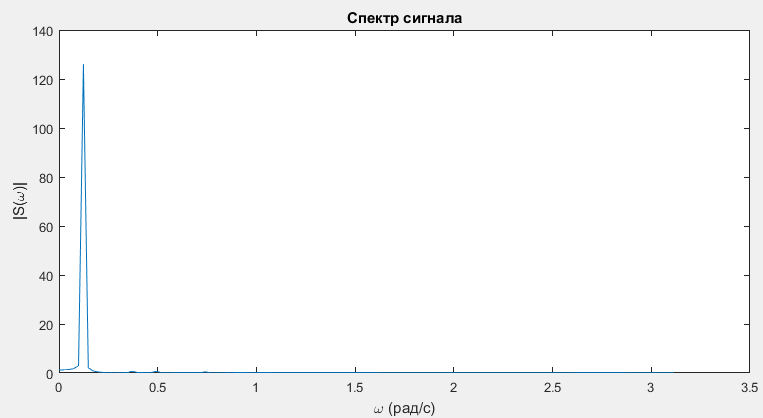
\includegraphics[scale=0.7]{phase_demod_sig_spec}
		\caption{Спектр фазово-демодулированного сигнала} 
		\label{pic:phase_demod_sig_spec} % название для ссылок внутри кода
	\end{center}
\end{figure}
\begin{figure}[H]
	\begin{center}
		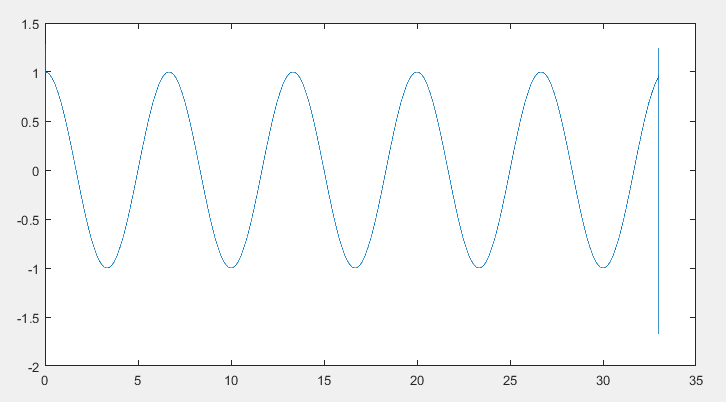
\includegraphics[scale=0.7]{freq_demod_sig}
		\caption{Частотно-демодулированный сигнал} 
		\label{pic:freq_demod_sig} % название для ссылок внутри кода
	\end{center}
\end{figure}
\begin{figure}[H]
	\begin{center}
		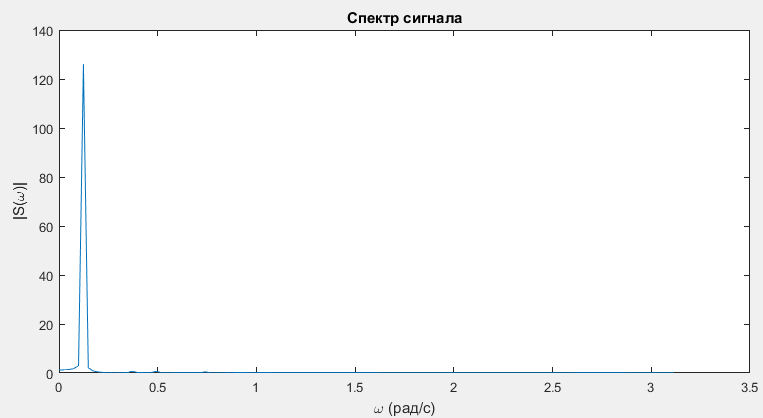
\includegraphics[scale=0.7]{freq_demod_sig_spec}
		\caption{Спектр частотно-демодулированного сигнала} 
		\label{pic:freq_demod_sig_spec} % название для ссылок внутри кода
	\end{center}
\end{figure}

В обоих случаях сигналы были восстановлены с высокой точностью.

\section{Выводы}

Исследованы типы аналоговой модуляции/демодуляции (фазовая, частотная). Построены спектры модулированных сигналов, их вид совпал с ожидаемым результатом для каждого типа модуляции.

Частотная модуляция применяется для высококачественной передачи звукового (низкочастотного) сигнала в радиовещании (в диапазоне УКВ), для звукового сопровождения телевизионных программ, передачи сигналов цветности в телевизионном стандарте SECAM, видеозаписи на магнитную ленту, музыкальных синтезаторах.
\end{document}
